\documentclass[11pt]{cernrep}
\usepackage{graphicx,epsfig}
\bibliographystyle{lesHouches}

\usepackage{xspace}
\newcommand{\Sherpa}{S\protect\scalebox{0.8}{HERPA}\xspace}
\newcommand{\Powheg}{P\protect\scalebox{0.8}{OWHEG}\xspace}
\newcommand{\CSS}{C\protect\scalebox{0.8}{SS}\xspace}
\newcommand{\Comix}{C\protect\scalebox{0.8}{OMIX}\xspace}
\newcommand{\Amegic}{A\protect\scalebox{0.8}{MEGIC++}\xspace}
\newcommand{\MCatNLO}{M\protect\scalebox{0.8}{C}@N\protect\scalebox{0.8}{LO}\xspace}
\newcommand{\MEPS}{M\scalebox{0.8}{E}P\scalebox{0.8}{S}\xspace}
\newcommand{\MEPSatNLO}{M\scalebox{0.8}{E}P\scalebox{0.8}{S}@N\protect\scalebox{0.8}{LO}\xspace}
\newcommand{\Collier}{C\protect\scalebox{0.8}{OLLIER}\xspace}
\newcommand{\OpenLoops}{O\protect\scalebox{0.8}{PEN}L\protect\scalebox{0.8}{OOPS}\xspace}
\newcommand{\Herwig}{H\protect\scalebox{0.8}{ERWIG}7\xspace}
\newcommand{\Matchbox}{M\protect\scalebox{0.8}{ATCHBOX}\xspace}
\newcommand{\MGaMC}{M\protect\scalebox{0.8}{AD}G\protect\scalebox{0.8}{RAPH}5\_aMC@NLO\xspace}
\newcommand{\MadGraph}{M\protect\scalebox{0.8}{AD}G\protect\scalebox{0.8}{RAPH}\xspace}
\newcommand{\MGAMC}{MG5\_aMC\xspace}
\newcommand{\MadGraphfour}{M\protect\scalebox{0.8}{AD}G\protect\scalebox{0.8}{RAPH}4\xspace}
\newcommand{\CVolver}{CV\protect\scalebox{0.8}{OLVER}\xspace}
\newcommand{\ColorFull}{C\protect\scalebox{0.8}{OLOR}F\protect\scalebox{0.8}{ULL}\xspace}
\newcommand{\MoCaNLO}{M\protect\scalebox{0.8}{oCaNLO}\xspace}
\newcommand{\Recola}{R\protect\scalebox{0.8}{ecola}\xspace}
\newcommand{\VBFNLO}{V\protect\scalebox{0.8}{BFNLO}\xspace}
\newcommand{\pt}{\ensuremath{p_{T}}\xspace}
\newcommand\sss{\mathchoice%
{\displaystyle}%
{\scriptstyle}%
{\scriptscriptstyle}%
{\scriptscriptstyle}%
}
\newcommand\MSB{\ifmmode {\overline{\rm MS}} \else $\overline{\rm MS}$\fi}
\newcommand\MINLO{{\tt MiNLO}}
\newcommand\muf{\mu_{\sss\rm F}}
\newcommand\mur{\mu_{\sss\rm R}}
\newcommand\KRA{K_{\scriptscriptstyle \rm R}}
\newcommand\KFA{K_{\scriptscriptstyle \rm F}}

\newcommand{\GOSAM}{G\protect\scalebox{0.8}{O}S\protect\scalebox{0.8}{AM}\xspace}
\newcommand{\POWHEGBOX}{P\protect\scalebox{0.8}{OWHEG} B\protect\scalebox{0.8}{OX}\xspace}
\newcommand{\QGRAF}{Q\protect\scalebox{0.8}{GRAF}\xspace}
\newcommand{\FORM}{F\protect\scalebox{0.8}{ORM}\xspace}
\newcommand{\SAMURAI}{S\protect\scalebox{0.8}{AMURAI}\xspace}
\newcommand{\GOLEM}{G\protect\scalebox{0.8}{OLEM}\xspace}
\newcommand{\NINJA}{N\protect\scalebox{0.8}{INJA}\xspace}
\newcommand{\SPINNEY}{S\protect\scalebox{0.8}{PINNEY}\xspace}
\newcommand{\ONELOOP}{O\protect\scalebox{0.8}{NE}LO\protect\scalebox{0.8}{OP}\xspace}
\newcommand{\MCFM}{M\protect\scalebox{0.8}{CFM}\xspace}

% Commands defined by Mathieu
\usepackage{amsmath}
\newcommand{\MP}[1]{{ {\color{blue}{ [MP: #1]}} }}
\newcommand{\KL}[1]{{ {\color{yellow}{ [KL: #1]}} }}
\newcommand{\SB}[1]{{ {\color{green}{ [SB: #1]}} }}
\newcommand{\MR}[1]{{ {\color{cyan}{ [MR: #1]}} }}

\usepackage{color}
\usepackage{morefloats}

\begin{document}

\section{Study of electroweak production of WZ in association with two jets at the LHC 
\protect\footnote{Section coordinators: K.~Long, M.~Pellen.}$^{,}$ 
\protect\footnote{Contributing authors: S.~Br\"auer, V.~Ciulli, S.~Gieseke, M.~Herndon, M.~Mozer, S.~Pl{\"a}tzer, M.~Rauch, E.~Yazgan.}$^{,}$
\protect\footnote{The work of SB is supported by German Federal Ministry for Education and Research (BMBF) under contract 05H15MGCAA.
MP acknowledges financial support by the BMBF under contract no.~05H15WWCA1 and the German Science Foundation (DFG) under reference number DE 623/6-1. 
EY is supported by Chinese Academy of Sciences (CAS), MoST (Ministry of Science and Technology) through project no.~2013CB837801, and NSFC (National Natural Science Foundation of China) through project no.~11661141007. 
\label{vbs_section}}}

\subsection{Introduction \label{vbs_intro}}

The electroweak (EW) production of vector-boson pairs in association with two jets at the CERN Large Hadron Collider (LHC) forms an important class of processes both theoretically and experimentally.
This signature includes vector-boson scattering (VBS) contributions, which constitute the principle example of processes where the scattering of two massive gauge bosons can be observed at the LHC.
These processes provide a natural probe of the vector-boson quartic couplings, which arise due to the non-Abelian nature of the electroweak gauge group and are exactly predicted in the Standard Model (SM).
The Higgs boson plays a unique role in these interactions, preventing the cross section from diverging in the high-energy limit and preserving the unitarity of the associated scattering amplitudes.
Deviations in these channels could therefore indicate physics beyond the SM in the electroweak sector.

The measurements of these processes are particularly challenging due to their high multiplicities and small cross sections.
They have been observed and even measured only recently by the experimental collaborations at the LHC.
The most precise current measurement \cite{Aad:2014zda,Khachatryan:2014sta,Sirunyan:2017ret,Aaboud:2016ffv} concerns the scattering of two same sign W bosons (usually denoted ${\rm W}^\pm{\rm W}^\pm{\rm j}{\rm j}$).
This process has a unique signature due to the same-sign charged leptons in the final state.
The cross section is well within reach with the large data sets being collected in the LHC Run II, and the
signature is experimentally accessible due to the precise lepton identification, charge assignment, and momentum resolution of the LHC experiments.
The nature of the final state is also attractive due to the low rate of background processes
producing two prompt, same sign leptons associated with forward jets (referred to as the irreducible background).

Measurements of other VBS signatures such as ${\rm Z}{\rm Z}{\rm j}{\rm j}$, ${\rm W}^+{\rm W}^-{\rm j}{\rm j}$, or ${\rm W}^{\pm}{\rm Z}{\rm j}{\rm j}$ present additional challenges due to the lower cross section and larger irreducible backgrounds, which dominate over the VBS contribution in most regions of phase space.
Nonetheless, studies have already been made at the LHC of both the ${\rm Z}{\rm Z}{\rm j}{\rm j}$ \cite{Sirunyan:2017fvv} and ${\rm W}^{\pm}{\rm Z}{\rm j}{\rm j}$ \cite{Aad:2016ett} signature at $\sqrt{s} = 8$~TeV.
In these cases, separation of the electroweak component of the $VV{\rm j}{\rm j}$ state depends on exploiting the different characteristics of the EW and non-EW components through kinematic selections.
Accurate predictions for discriminating distributions and a detailed understanding of their associated uncertainties therefore directly impact such measurements.
A theory-agnostic measurement that does not attempt separation of states by production mode avoids such dependencies,
but cannot fully leverage the statistical tools and treatment of uncertainties available in an experimental analysis.
The approaches are therefore complementary, and are often presented together in experimental results.

From a theoretical point of view, one of the challenges for the predictions of the EW di-boson production in association with two jets is its high multiplicity.
This is why in the past, next-to-leading order (NLO) predictions have focused on VBS approximations.
Only recently, full NLO computations became available at NLO QCD and EW for both the EW component and the QCD-induced process for ${\rm W}^\pm{\rm W}^\pm{\rm j}{\rm j}$ \cite{Biedermann:2017bss}.
For this process, preliminary results \cite{Anders:2018gfr} of a comparison of different theoretical predictions have shown that differences between the full computation and VBS-approximated ones are not significant given the present experimental accuracy.
Qualitatively, one could expect a similar conclusion for other processes such as ${\rm W}^{\pm}{\rm Z}{\rm j}{\rm j}$ but a quantitative check is still needed.
Therefore, in these proceedings we aim at making a similar comparison of theoretical predictions implemented in Monte Carlo programs.
This allows to infer the quality of the VBS approximation at leading-order (LO).

As such there is strong motivation for an investigation of the theoretical predictions, tools, and uncertainties used in a typical VBS analysis. 
We focus on the ${\rm W}^{\pm}{\rm Z}{\rm j}{\rm j}$ \cite{Aad:2016ett} state, the measurement of which is strongly limited by the size of the data set, 
but which has not yet been studied at the 13 TeV LHC. Hence, a preliminary study on this process is of particular interest.

Due to its colour structure, the ${\rm W}^{\pm}{\rm Z}{\rm j}{\rm j}$ signature possesses three different contributions at LO.
The first, of order $\mathcal{O} (\alpha^6)$, is usually referred to as the EW component or even VBS component (even if it also possesses non-VBS contributions such as tri-boson production).
The two quark lines can also be connected via a gluon while the gauge bosons are radiated off the quark lines.
This contribution is of order $\mathcal{O} (\alpha_{\rm s}^2\alpha^4)$ and is called QCD contribution/background.
Finally, there exists a non-zero interference of order $\mathcal{O} (\alpha_{\rm s}\alpha^5)$.
For this signature (as opposed to \emph{e.g.}\ ${\rm W}^\pm{\rm W}^\pm{\rm j}{\rm j}$) the EW component is highly suppressed with respect to the QCD one.
This implies having very exclusive experimental cuts in order to enhance the EW contribution and a good control over the description of both the EW signal and QCD background.
To that end, the understanding of theoretical predictions and Monte Carlo programs is key.
In particular, it is vital to ensure that all different programs can provide equivalent physics result.
Such comparisons can also shed light on the true uncertainties of such predictions.
Typically, uncertainty treatments asses the impact of parton density function (PDF) uncertainties or of missing higher orders in perturbative QCD.
But in addition, Monte Carlo generators require many input parameters and the selection of which can have a significant impact on the predictions both in shape and normalisation.
In the present study we use a common set-up for all predictions at LO accuracy. We additionally provide results with
variations in some parameters and comment on their effects and motivations.

In these proceedings, we start with Sec.~\ref{vbs_theory} where a short review of the theoretical state-of-the-art predictions is given.
The programs used in the present work are also briefly described.
In Sec.~\ref{setup}, the set-up of the calculation is presented.
It amounts to give the input parameters as well as the event selection.
Section~\ref{vbs_results} is devoted to the results of the study.
It starts with LO predictions for the three different contributions to the ${\rm e}^+  \nu_{\rm e}  \mu^+ \mu^- {\rm j} {\rm j}$ final state at the LHC.
Then the various comparisons are reported at both fixed-order and with parton shower.
Finally, Sec.~\ref{vbs_concl} contains a summary, concluding remarks as well as recommendations.

\subsection{Theory and event generators \label{vbs_theory}}

The study focuses on the ${\rm W}^{\pm}{\rm Z}{\rm j}{\rm j}$ signature and more precisely on the partonic processes

\begin{equation}
 {\rm p} {\rm p} \to {\rm e}^+  \nu_{\rm e}  \mu^+ \mu^- {\rm j} {\rm j} ,
\end{equation}
%
and
%
\begin{equation}
 {\rm p} {\rm p} \to {\rm e}^-  \bar \nu_{\rm e}  \mu^+ \mu^- {\rm j} {\rm j}.
\end{equation}
%
The predictions presented are all at LO but NLO QCD corrections to the EW contribution and its irreducible background are known since 10 years in the VBS approximation \cite{Bozzi:2007ur} while the QCD corrections to the QCD-induced process have been computed more recently \cite{Campanario:2013qba}.
The NLO EW corrections are currently unknown.
In Ref.~\cite{Biedermann:2016yds}, it has been argued that large NLO EW corrections to the EW contributions are an intrinsic feature of VBS at the LHC.
Therefore, they are expected to play a significant role for all VBS signatures.
In Ref.~\cite{Biedermann:2017bss}, which focuses on the computation of the full NLO corrections to the ${\rm W}^\pm{\rm W}^\pm{\rm j}{\rm j}$ process, it has been shown that the EW corrections to the EW process are the dominant NLO corrections.
This means that the EW corrections to the EW contributions are expected to be at least of the same order as the QCD corrections for other VBS signatures.
Parton-shower effects to VBS processes and the resulting uncertainties
induced by a variation of factorisation, renormalisation, and
shower-starting scale have also been studied
recently~\cite{Rauch:2016upa,Rauch:2016pai}, taking the ${\rm W}^+{\rm
W}^-{\rm j}{\rm j}$ VBS process as an example. Thereby, the standard LHC
jet definition with a cone radius of $R{=}0.4$ leads to migration
effects~\cite{Rauch:2017cfu} and a reduction of the cross section by about $10\%$ compared to
the fixed-order results after VBS cuts.

In the following, the codes used for the predictions are briefly described.

\subsubsection*{\protect\MGaMC \label{vbs_mgamc}}

{\sc MadGraph5\_aMC@NLO}~\cite{Alwall:2014hca} is an automatic meta-code (a code that generates codes) which makes it possible to simulate any scattering process
      including NLO QCD corrections both at fixed-order and including matching to parton showers. 
      The commands that have been used for the present computation (for the W$^{-}$ case) are 
\begin{verbatim}
> set complex_mass_scheme
> set gauge Feynman
> generate p p > e- ve~ mu+ mu- j j QED=6 QCD=0
> output WmZJJToENu2MuJJ
\end{verbatim}
  The version used is 2.6.0. We use the complex mass scheme and Feynman gauge for consistency with \MoCaNLO+\Recola, but 
  verify that we obtain equivalent results if they are not explicity specified.
  We note that the ``deltaeta'' variable in the MG5\_aMC run\_card also applies a requirement that the two jets
  have opposite rapidity sign. We do not make this requirement for our fidicual region definition, so we remove this condition for our comparisons.
  This is accomplished by modifying the cut behaviour in cuts.f in the ``SubProcesses'' folder, and validated by
  generating events without this condition and applying selections to the LHE-level partons using standalone code.
%   Note that alternatively, we have tested the following commands
%   \begin{verbatim}
% > set gauge Feynman
% > set complex_mass_scheme
% > generate p p > e+  ve  mu+ mu- j j QCD^2==0 QED^2==12
% > output WpZJJToENu2MuJJ_bis
% \end{verbatim}
%   with the version 2.5.1.
%   These commands gave for the cross section with our common set-up: $0.2861(8)$~fb.
% Results are statistically equivalent and are now understood to be related to the deltaeta cut discussed
  
\subsubsection*{\protect\Herwig \label{vbs_herwig}}

Based on extensions of the previously developed \Matchbox
module~\cite{Platzer:2011bc}, the \Herwig event generator~\cite{Bellm:2015jjp,Bahr:2008pv} facilitates the automated set-up of all ingredients necessary for a full NLO QCD calculation.
It relies on an implementation of the Catani--Seymour dipole
subtraction method~\cite{Catani:1996vz,Catani:2002hc}, as well as
interfaces to a list of external matrix element providers -- either
at the level of squared matrix elements, based on extensions of the
BLHA standard~\cite{Binoth:2010xt,Alioli:2013nda,Andersen:2014efa} or
at the level of colour-ordered sub-amplitudes.

For this study the relevant tree-level matrix elements have been
provided by an interface to VBFNLO \cite{Arnold:2008rz,Arnold:2011wj,Baglio:2014uba} using an extension of the BLHA
accord. We have matched these calculations to the angular ordered
shower using the subtractive matching and default settings of the
\Herwig~7.1 release. The PDF sets that have been used to tune the parton shower are MMHT2014lo68cl and
MMHT2014nlo68cl~\cite{Harland-Lang:2014zoa}.
These sets are not the one used for this computation (see below).
This can in particular impact initial-state radiations.
We consider variations of the hard shower scale as detailed in Ref.~\cite{Bellm:2016rhh}, using the 'resummation' profile scale choice.

\subsubsection*{\protect{\MoCaNLO\!+\Recola} \label{vbs_MoCaNLO_Recola}}

The program {\sc MoCaNLO+Recola} is made of a flexible Monte Carlo program dubbed {\sc MoCaNLO} and of the general matrix element generator {\sc Recola}~\cite{Actis:2012qn,Actis:2016mpe}.
The program can compute arbitrary processes in the Standard Model with NLO QCD and EW accuracy.
The fast integration is ensured by using similar phase-space mappings to those of Refs.~\cite{Berends:1994pv,Denner:1999gp,Dittmaier:2002ap}.
The complex-mass scheme~\cite{Denner:1999gp,Denner:2005fg} to treat unstable particles is always used.
These tools have been successfully used for the computation of NLO corrections for high-multiplicity processes and in particular VBS processes \cite{Biedermann:2016yds,Biedermann:2017bss}.

\subsubsection*{\protect\Sherpa \label{vbs_sherpa}}
\Sherpa~\cite{Gleisberg:2008ta,Gleisberg:2003xi} is a multipurpose event generator for high-energy particle collisions. 
It is built out of several algorithms and modules tailored to many different physics challenges of collider physics.
In the \Sherpa framework the infrared divergences appearing in the real-emission are treated by the Catani--Seymour dipole-subtraction method~\cite{Catani:1996vz,Catani:2002hc,Gleisberg:2007md}. 
The default parton-shower algorithm of \Sherpa is based on the Catani--Seymour factorisation~\cite{Schumann:2007mg,Hoeche:2009xc}.
For NLO computations, interfaces to several one-loop generators exist, with the interface to \textsc{Recola}~\cite{Actis:2012qn,Actis:2016mpe} being the latest addition~\cite{Biedermann:2017yoi}.
For correctly combining the matrix elements in multijet-production processes with the parton shower, \Sherpa has adapted the MEPS@LO method~\cite{Hoeche:2009rj} at LO and its generalisation MEPS@NLO~\cite{Hoche:2010kg} at NLO. 
In this study, the matrix elements are provided by \textsc{Comix}~\cite{Gleisberg:2008fv}, one of the two built-in generators next to \textsc{Amegic}~\cite{Krauss:2001iv}.
Both of the studied partonic processes are then showered with the default shower.

\subsubsection*{\protect\VBFNLO \label{vbs_VBFNLO}}
\VBFNLO~\cite{Arnold:2008rz,Arnold:2011wj,Baglio:2014uba} is a flexible
Monte-Carlo event generator for processes with electroweak bosons.
Besides the Standard Model, selected processes can also be calculated in
a variety of new-physics models, including effective field theories with
dimension-6 and dimension-8 operators.
The matrix elements for VBF and VBS processes are calculated in the VBS
approximation. The corresponding $s$-channel contribution, which can be
seen as triboson production where one vector boson decays hadronically,
is available as well, but its contribution not included in the studies
presented here.
Its use of leptonic tensors in the calculation of the matrix elements
can lead to a significant speed improvement compared to automatically
generated code.
For results with parton showers in this study, \VBFNLO can serve as the
matrix-element provider and phase-space generator for \Herwig. The
interface between the two programs is based on an extension of the BLHA
standard~\cite{Binoth:2010xt,Alioli:2013nda,Andersen:2014efa}. When
combining \VBFNLO results with showering performed by Pythia, event
files following the Les Houches LHE file
standard~\cite{Boos:2001cv,Alwall:2006yp} are used instead.


\subsection{Details of the set-up \label{setup}}

In this section we describe default input parameters that have been used.
Also, the event selection used in the comparison is described.

\subsubsection*{Input parameters}

All simulations are performed for the LHC running with a center-of-mass energy $\sqrt s = 13 {\rm~TeV}$.
The default PDF used is the NNPDF~3.0 set~\cite{Ball:2014uwa} with four active flavour at LO and a strong coupling constant $\alpha_{\rm s}\left( M_{\rm Z} \right) = 0.130$.\footnote{Its {\tt lhaid} in LHAPDF6~\cite{Buckley:2014ana} is 263400.} 
% NNPDF30_lo_as_0130_nf_4 
If this default PDF is not employed, it is explicitly stated.
%
The masses and widths of the particle used in the simulations are
%
\begin{alignat}{2}
                M_{\rm t}   &=  173.21 {\rm~GeV},             & \quad \quad \quad \Gamma_{\rm t} &= 0 {\rm~GeV},  \nonumber \\
                M_{\rm Z}^{\rm OS} &=  91.1876{\rm~GeV},      & \quad \quad \quad \Gamma^{\rm OS}_{\rm Z} &= 2.4952{\rm~GeV},  \nonumber \\
                M_{\rm W}^{\rm OS} &=  80.385{\rm~GeV},       & \Gamma^{\rm OS}_{\rm W} &= 2.085{\rm~GeV},  \nonumber \\
                M_{\rm H} &=  125.0{\rm~GeV}, 		      & \Gamma_{\rm H}   &=  4.07 \times 10^{-3}{\rm~GeV}.
\end{alignat}
%
The value of the mass and width of the Higgs boson are those recommended by the Higgs cross section working group \cite{deFlorian:2016spz}.
The top quark does not appear at tree level in the simulations when the bottom-quarks in the initial state are neglected.
Therefore its width is set to zero.
The numerical values used in the simulation for the pole mass/width of the gauge bosons ($V={\rm W,Z}$) are obtained from the measured on-shell (OS) values for the masses and widths according to Ref.~\cite{Bardin:1988xt} as:
%
\begin{equation}
        M_V = M_{\rm V}^{\rm OS}/\sqrt{1+(\Gamma_{\rm V}^{\rm OS}/M_{\rm V}^{\rm OS})^2}\,,\qquad  \Gamma_V = \Gamma_{\rm V}^{\rm OS}/\sqrt{1+(\Gamma_{\rm V}^{\rm OS}/M_{\rm V}^{\rm OS})^2}.
\end{equation}
%
The EW coupling is renormalised in the $G_\mu$ scheme \cite{Denner:2000bj} where
%
\begin{equation}
    G_{\mu}    = 1.16637\times 10^{-5}{\rm~GeV}^{-2}.
\end{equation}
%
The input parameters above yield a numerical value for $\alpha$ of
%
\begin{equation}
 \alpha = 7.555310522369 \times 10^{-3}.
\end{equation}
%
Note that for the EW contribution of order $\mathcal{O} (\alpha^6)$, no dependence on the strong coupling appears.
For contributions (interference or QCD-induced contributions) where there is a dependence on $\alpha_{\rm s}$, the numerical value used is the one extracted from the PDF set.

For the renormalisation and factorisation scales, two choices have been adopted.
For the fixed scale, it is
%
\begin{equation}
 \mu = \mu_{\rm fix} = M_{\rm W},
\end{equation}
%
while the dynamical scale used is
%
\begin{equation}
 \mu = \mu_{\rm dyn} = {\rm Max}\left[p_{\rm T, j}\right].
\end{equation}
%
The latter should be understood as the maximum of the transverse momenta of the tagging jets (defined below).
This observable is closely connected to the momentum transfer through
the virtual vector boson, which has been shown to be a reasonable scale
choice, and is also a reasonable choice when used as the starting scale
of the parton shower~\cite{Rauch:2016upa}.
These two scales are the default fixed and dynamical scale, respectively.
If the scale used is different, this is explicitly stated in the text.

Photon-induced as well as bottom-induced contributions have been neglected.
The photon contributions are expected to be small \cite{Biedermann:2017bss} while the bottom-induced contribution can lead to single-top resonant contributions.
The later can in principle be isolated thanks to kinematical constraints.

\subsubsection*{Event selection}

Following experimental studies \cite{Aad:2016ett,CMS-PAS-SMP-14-008}, the event selection used for the present work is:

\begin{itemize}
\item All charged leptons are required to have
    \begin{align}
        \label{cut:1}
         p_{\rm T, \ell} >  20{\rm~GeV},\qquad |y_{\ell}| < 2.5.
    \end{align}
\item For the leptons of opposite charge and same flavour, an invariant mass cut to single out the Z-boson resonance is applied:
    \begin{align}
        \label{cut:2}
         76 {\rm~GeV} < m_{l_i^+ l_i^-} < 106 {\rm~GeV}.
    \end{align}

\item QCD jets are clustered thanks to the anti-$k_T$ algorithm~\cite{Cacciari:2008gp} with radius parameter $R=0.4$.
      At least two jets are required to have
        \begin{align}
        \label{cut:3}
         p_{\rm T, j} >  30{\rm~GeV}, \qquad |y_{\rm j}| < 4.7, \qquad \Delta R_{\rm j \ell} > 0.4,
        \end{align}
        %
        and are called tagging jets.
\item On the two leading tagging jets, typical VBS cuts are applied:
        \begin{align}
        \label{cut:4}
         m_{\rm j j} >  500{\rm~GeV},\qquad |\Delta y_{\rm j j}| > 2.5.
        \end{align}
\end{itemize}

These cuts have been issued either directly in the Monte Carlo programs or using a {\sc Rivet} routine \cite{Buckley:2010ar}.
This file will be made public in order to make the present study easily reproducible.

\subsection{Results \label{vbs_results}}

\subsubsection*{Several contributions for one process}

As explained previously, the processes ${\rm p} {\rm p} \to {\rm e}^+  \nu_{\rm e}  \mu^+ \mu^- {\rm j} {\rm j}$  and ${\rm p} {\rm p} \to {\rm e}^-  \bar \nu_{\rm e}  \mu^+ \mu^- {\rm j} {\rm j}$
possess at LO three contributions of orders $\mathcal{O} (\alpha^6)$, $\mathcal{O} (\alpha_{\rm s}\alpha^5)$, and $\mathcal{O} (\alpha_{\rm s}^2\alpha^4)$.
As it can be seen in Table~\ref{table:xsectallLOdyn}, the EW component represents only about $20\%$ of the total cross section\footnote{In this subsection and in particular for the results of Table~\ref{table:xsectallLOdyn} and Fig.~\ref{fig:diffcontr}, the cut $|y_{\rm j}| < 4.5$ as been used instead of $4.7$ as everywhere else. This has a $1\%$ effect on the fiducial cross section.}.
This is in contrast with the ${\rm W}^\pm{\rm W}^\pm{\rm j}{\rm j}$ signature where the EW component represents almost $90\%$ of the cross section \cite{Biedermann:2017bss} in a comparable fiducial volume.
Hence measuring the EW component is much more challenging.
Therefore, inferring the shape of the signal and irreducible background is key.
Note that the interference contribution is about $0.5\%$ which is negligible with respect to current experimental accuracy.\footnote{For the ${\rm W}^\pm{\rm W}^\pm{\rm j}{\rm j}$ signature, the interference contribution has been shown to be around $3\%$ \cite{Biedermann:2017bss}.}

\begin{table}
\begin{center} 
\begin{tabular}{ c | c | c }
 $\mu = \mu_{\rm dyn}$ / $\sigma_{\rm LO}$ [fb] & ${\rm p} {\rm p} \to {\rm e}^+  \nu_{\rm e}  \mu^+ \mu^- {\rm j} {\rm j}$  & ${\rm p} {\rm p} \to {\rm e}^-  \bar \nu_{\rm e}  \mu^+ \mu^- {\rm j} {\rm j}$  \\
  \hline\hline
  $\mathcal{O} (\alpha^6)$                        & $0.25416(6)$  & $0.15003(3)$   \\
  $\mathcal{O} (\alpha_{\rm s}\alpha^5)$          & $0.006833(6)$ & $0.003977(3)$  \\
  $\mathcal{O} (\alpha_{\rm s}^2\alpha^4)$        & $0.9912(2)$   & $0.6306(6)$   \\
  \hline
\end{tabular}
\end{center}
\caption{
Fiducial cross sections at LO for the process ${\rm p}{\rm p}\to{\rm e}^+\nu_{\rm e}\mu^+\mu^-{\rm j}{\rm j}$ and ${\rm p}{\rm p}\to{\rm e}^-\bar\nu_{\rm e}\mu^+\mu^-{\rm j}{\rm j}$ at orders $\mathcal{O} (\alpha^6)$, $\mathcal{O} (\alpha_{\rm s}\alpha^5)$, and $\mathcal{O} (\alpha_{\rm s}^2\alpha^4)$.
The predictions are expressed in fb and are for the LHC running at a centre-of-mass energy of $\sqrt{s}=13 {\rm~TeV}$.
The scale used in the simulations is $\mu = \mu_{\rm dyn} = {\rm Max}\left[p_{\rm T, j}\right]$.
The integration errors of the last digits are given in parentheses.}
\label{table:xsectallLOdyn}
\end{table}

In Fig.~\ref{fig:diffcontr}, several differential distributions are shown.
In the upper plot the absolute predictions for each component as well as their sum are displayed.
In the lower plot, each contribution is normalised to their sum and expressed in per cent.
These distributions reflect the same conclusion as for the cross section namely that the processes are largely dominated by QCD-induced contribution.
The first two observables displayed (top) are the invariant mass and the rapidity difference of the two tagging jets.
These two observables are used as cuts [see Eq.~\eqref{cut:4}] in order to enhance the EW component over the QCD background.
The cuts are clearly visible on the plots and it is easily understandable why they are enhancing the EW contribution.
Toward high invariant-mass, the EW component becomes more and more important.
It even becomes of the same size as the QCD one for an invariant-mass of $2000{\rm~GeV}$.
The same holds true for high rapidity separation for the two jets.
On the other hand, the transverse invariant mass (bottom left) of muon--anti-muon pair does not display significant differences in the different contributions over the whole range.
Other transverse-momentum distributions display the same pattern.
Finally, we show the distance between the two jets.
This observable also seems to possess a good discriminating power.
In particular, for large distances, the EW component becomes dominant but with very low statistics.
The interference effects are extremely suppressed due to the smallness of the cross section.
Contribution of each of the studied observable does not exceed the per-cent level over the whole phase-space range.

\begin{figure}[htbp]
\begin{center}
   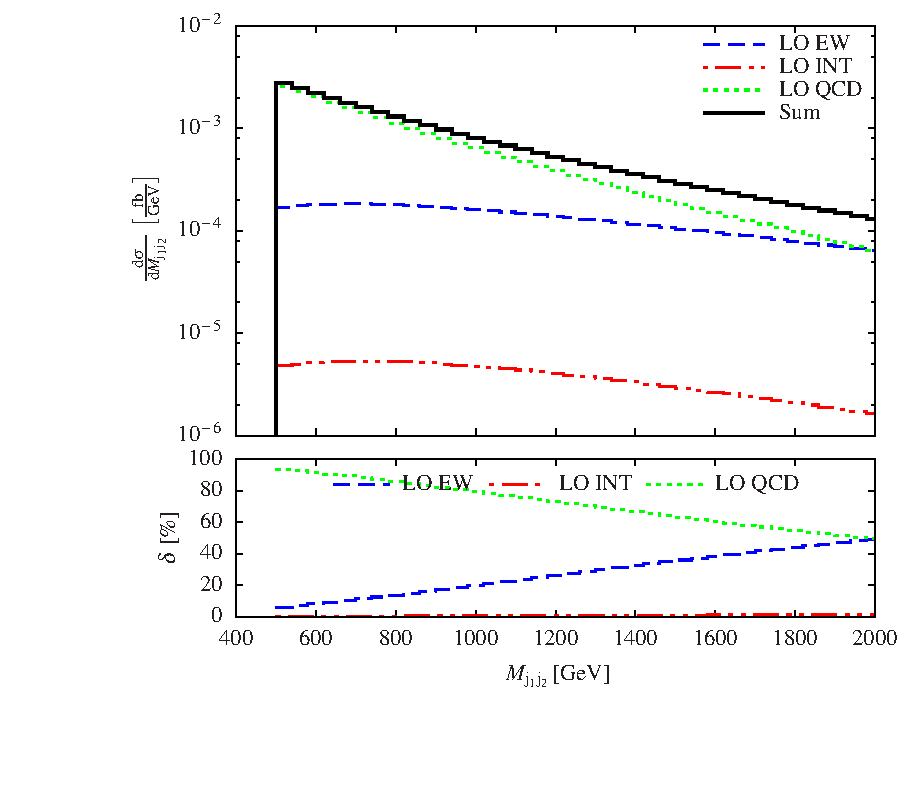
\includegraphics[scale=0.5]{figs/histogram_invariant_mass_mjj12}
   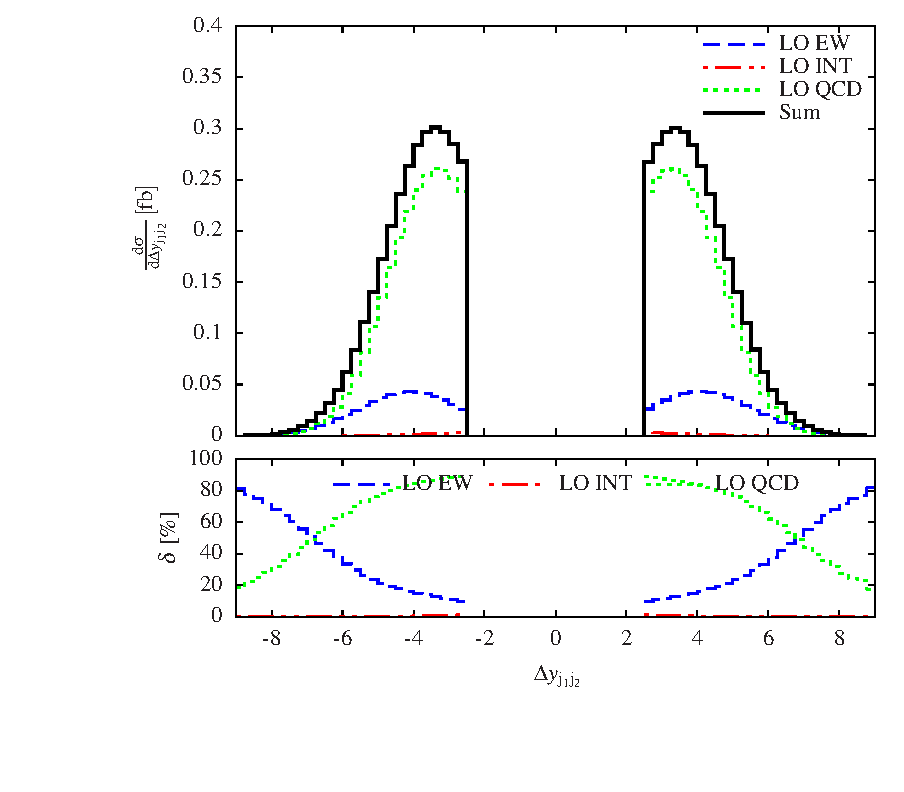
\includegraphics[scale=0.5]{figs/histogram_rapidity_separation_j1j2}
   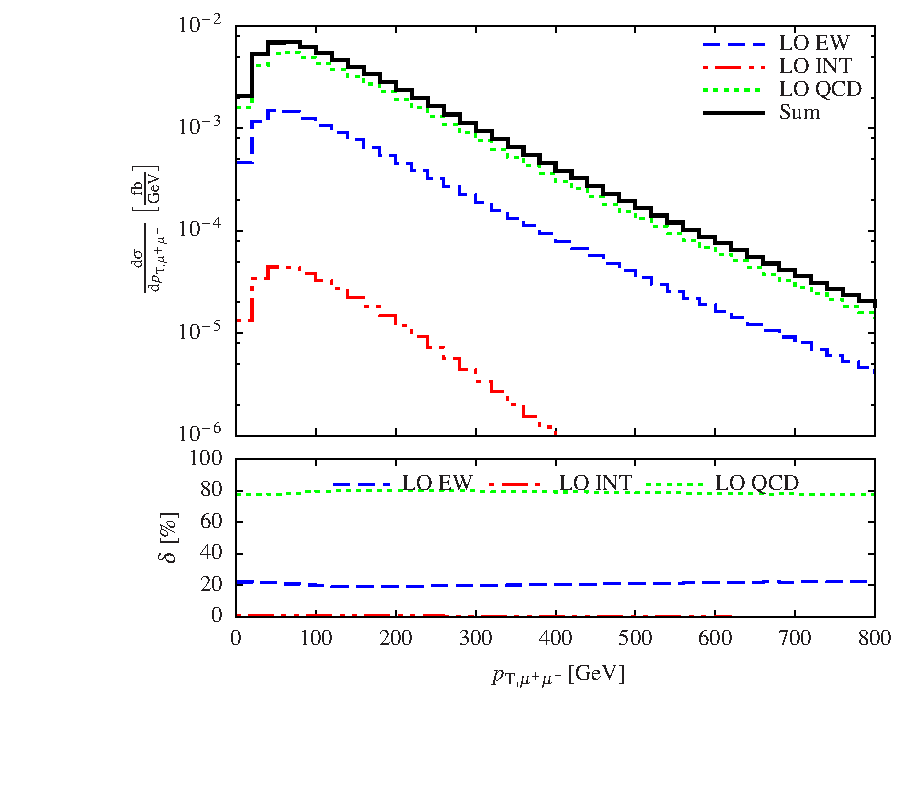
\includegraphics[scale=0.5]{figs/histogram_transverse_momentum_muamu}
   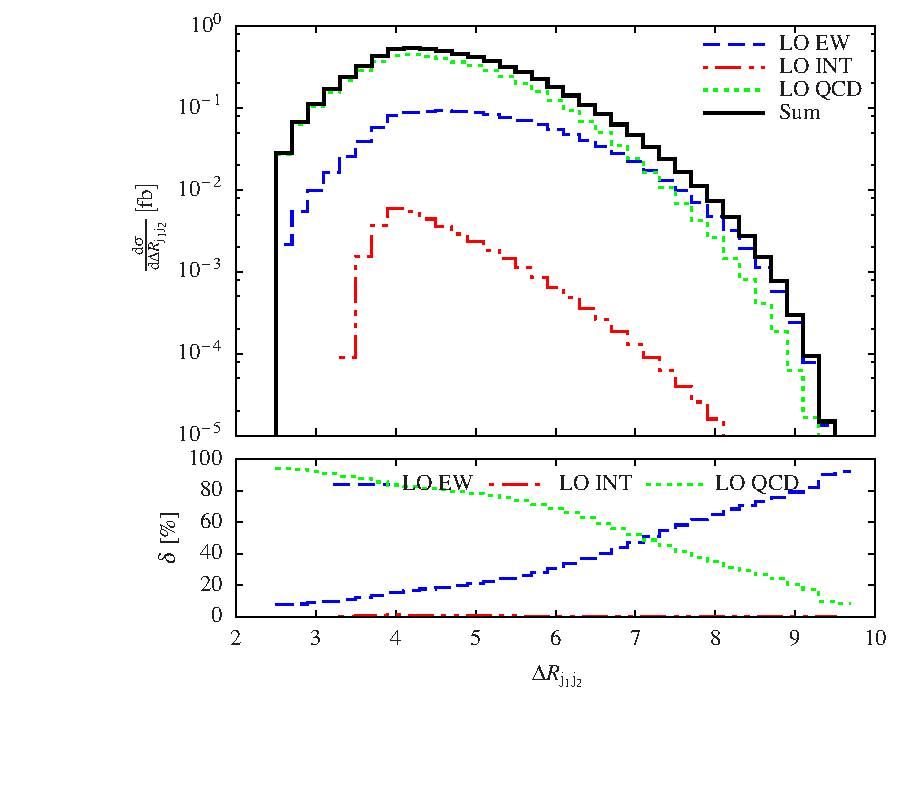
\includegraphics[scale=0.5]{figs/histogram_distance_djj12}
\caption{Differential distributions at a centre-of-mass energy $\sqrt{s}=13{\rm~TeV}$ at the LHC for ${\rm p} {\rm p} \to {\rm e}^+  \nu_{\rm e}  \mu^+ \mu^- {\rm j} {\rm j}$ 
with the contributions at orders $\mathcal{O} (\alpha^6)$ (EW), $\mathcal{O} (\alpha_{\rm s}\alpha^5)$ (INT), and $\mathcal{O} (\alpha_{\rm s}^2\alpha^4)$ (QCD): 
                invariant mass of the two jets~(top left),
                rapidity separation between the two jets~(top right)
                transverse momentum of the anti-muon--muon system~(bottom left), and
                distance between the two jets~(bottom right).
                The upper panels show the LO predictions as well as their sum.
                The lower panels display the respective contributions normalised to their sum.}
\label{fig:diffcontr}
\end{center}
\end{figure}

\subsubsection*{Parton level comparisons}

We start the comparison of the various predictions by a comparison at the level of the cross section.
The fiducial volume is the one described in Eqs.~\eqref{cut:1}-\eqref{cut:4}.
The results are documented in Tables~\ref{table:xsectLOfix} and \ref{table:xsectLOdyn}.
There, the cross sections for both processes ${\rm p} {\rm p} \to {\rm e}^+  \nu_{\rm e}  \mu^+ \mu^- {\rm j} {\rm j}$ and ${\rm p} {\rm p} \to {\rm e}^-  \bar \nu_{\rm e}  \mu^+ \mu^- {\rm j} {\rm j}$ at fixed and dynamical scales are presented.
In general, the predictions of \MoCaNLO\!+\Recola and \Sherpa are in perfect agreement while the ones of \MGaMC are showing some slight statistical disagreement but only for the fixed scale.
There, the difference between \MoCaNLO\!+\Recola/\Sherpa and \MGaMC is about a per cent as it can be seed in Table~\ref{table:xsectLOfix}.
% For the fixed scale displayed in , the largest difference is between the predictions of \MoCaNLO\!+\Recola and \Sherpa and amounts to $1.2\%$.
On the other hand, the predictions predictions of \VBFNLO are not expected to be in perfect agreement with the others as \VBFNLO is not using full matrix elements but VBS-approximated ones.
Nonetheless, the difference between the \VBFNLO predictions and the ones of \MoCaNLO\!+\Recola/\Sherpa amounts to $0.6\%$ for the fixed scale.

\begin{table}
\begin{center} 
\begin{tabular}{ c | c | c }
 $\mu = \mu_{\rm fix}$ / $\sigma_{\rm LO}^{\rm EW}$ [fb] & ${\rm p} {\rm p} \to {\rm e}^+  \nu_{\rm e}  \mu^+ \mu^- {\rm j} {\rm j}$  & ${\rm p} {\rm p} \to {\rm e}^-  \bar \nu_{\rm e}  \mu^+ \mu^- {\rm j} {\rm j}$  \\
  \hline\hline
  \MGaMC                  & $0.2857(8)$     & $0.1657(4)\phantom{0}$   \\
  {\sc MoCaNLO}+{\sc Recola}      & $0.2885(1)$     & $0.16718(3)$  \\
  {\sc Sherpa}                    & $0.2885(2)$     & $0.1670(2)\phantom{0}$   \\
  {\sc VBFNLO}                    & $0.2867(5)$     & $0.1661(3)\phantom{0}$   \\
  \hline
\end{tabular}
\end{center}
\caption{
Fiducial cross sections at LO for the process ${\rm p}{\rm p}\to{\rm e}^+\nu_{\rm e}\mu^+\mu^-{\rm j}{\rm j}$ and ${\rm p}{\rm p}\to{\rm e}^-\bar\nu_{\rm e}\mu^+\mu^-{\rm j}{\rm j}$ at order $\mathcal{O} (\alpha^6)$.
The predictions are expressed in fb and are for the LHC running at a centre-of-mass energy of $\sqrt{s}=13 {\rm~TeV}$.
The scale used in the simulations is $\mu = \mu_{\rm fix} = M_W$.
The integration errors of the last digits are given in parentheses.}
\label{table:xsectLOfix}
\end{table}

\begin{table}
\begin{center} 
\begin{tabular}{ c | c | c }
 $\mu = \mu_{\rm dyn}$ / $\sigma_{\rm LO}^{\rm EW}$ [fb] & ${\rm p} {\rm p} \to {\rm e}^+  \nu_{\rm e}  \mu^+ \mu^- {\rm j} {\rm j}$  & ${\rm p} {\rm p} \to {\rm e}^-  \bar \nu_{\rm e}  \mu^+ \mu^- {\rm j} {\rm j}$  \\
  \hline\hline
  \MGaMC                  & $0.2550(8)$  & $0.1492(5)\phantom{0}$ \\
  {\sc MoCaNLO}+{\sc Recola}      & $0.2574(2)$  & $0.15003(3)$  \\
  {\sc Sherpa}                    & $0.2574(2)$  & $0.14998(6)$   \\
%{\sc VBFNLO}                      & $XX$  & $XX$   \\
  \hline
\end{tabular}
\end{center}
\caption{
Fiducial cross sections at LO for the process ${\rm p}{\rm p}\to{\rm e}^+\nu_{\rm e}\mu^+\mu^-{\rm j}{\rm j}$ and ${\rm p}{\rm p}\to{\rm e}^-\bar\nu_{\rm e}\mu^+\mu^-{\rm j}{\rm j}$ at order $\mathcal{O} (\alpha^6)$.
The predictions are expressed in fb and are for the LHC running at a centre-of-mass energy of $\sqrt{s}=13 {\rm~TeV}$.
The scale used in the simulations is $\mu = \mu_{\rm dyn} = {\rm Max}\left[p_{\rm T, j}\right]$.
The integration errors of the last digits are given in parentheses.}
\label{table:xsectLOdyn}
\end{table}

As it can be seen in Fig.~\ref{vbs_fig_fixed_order}, where the invariant mass and rapidity separation of the two tagging jets are displayed, the agreement between the predictions is good in both shape and normalisation.
For the jet rapidity separation, all predictions agree within statistical uncertainties over the whole range, with some small normalisation differences. For the di-jet mass, statistically significant differences are more pronounced towards higher masses between \MGaMC and other generators. This difference was not fully understood, but could be attributed to undestimation of statistical uncertainties or subtle configuration differences.
% The larger discrepancy is found in the region of low rapidity-separation between the two jets.
% The difference is the largest between {\sc MoCaNLO}+{\sc Recola}/{\sc VBFNLO} and \MGaMC.
% This reflects what has already been seen at the level of the cross section. 

\begin{figure}[htbp]
\begin{center}
   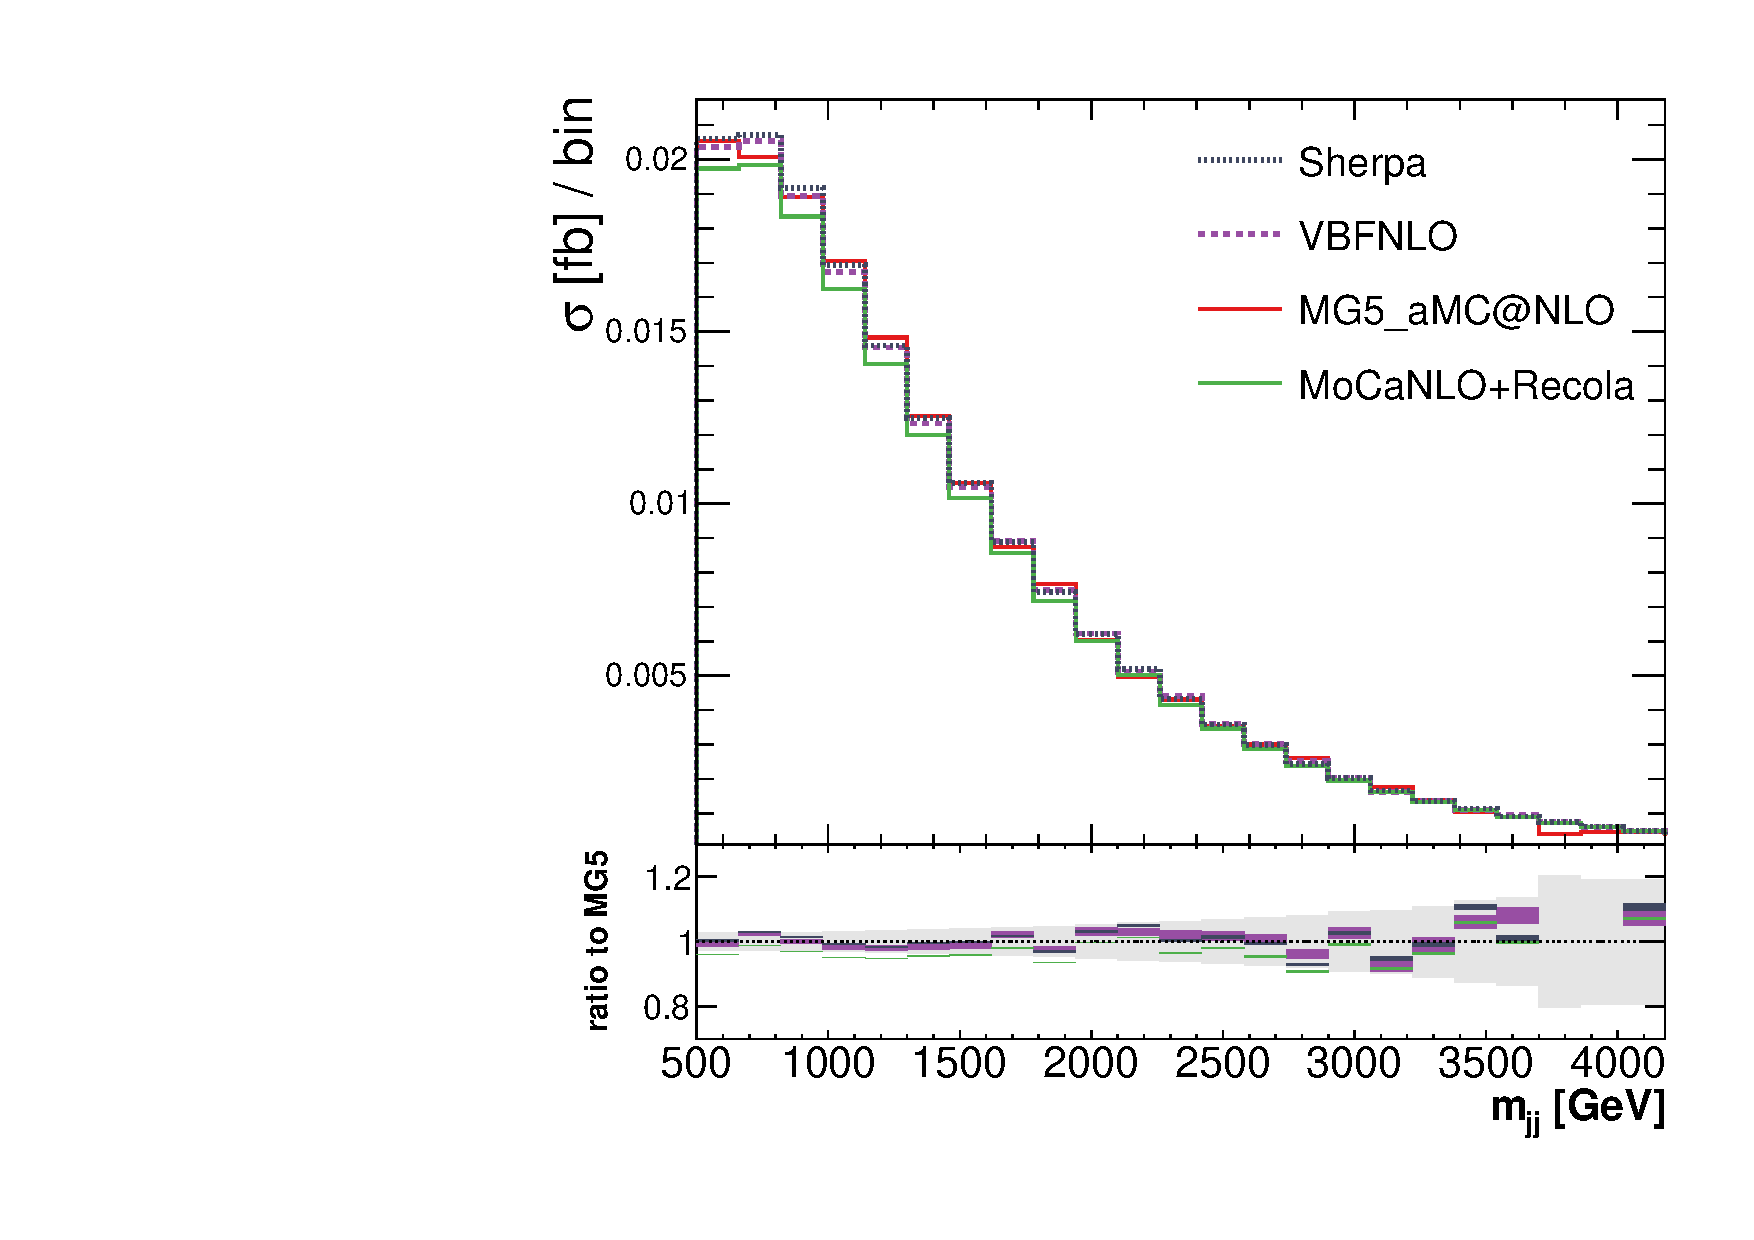
\includegraphics[scale=0.375]{figs/mjj_FixedOrder.pdf}
   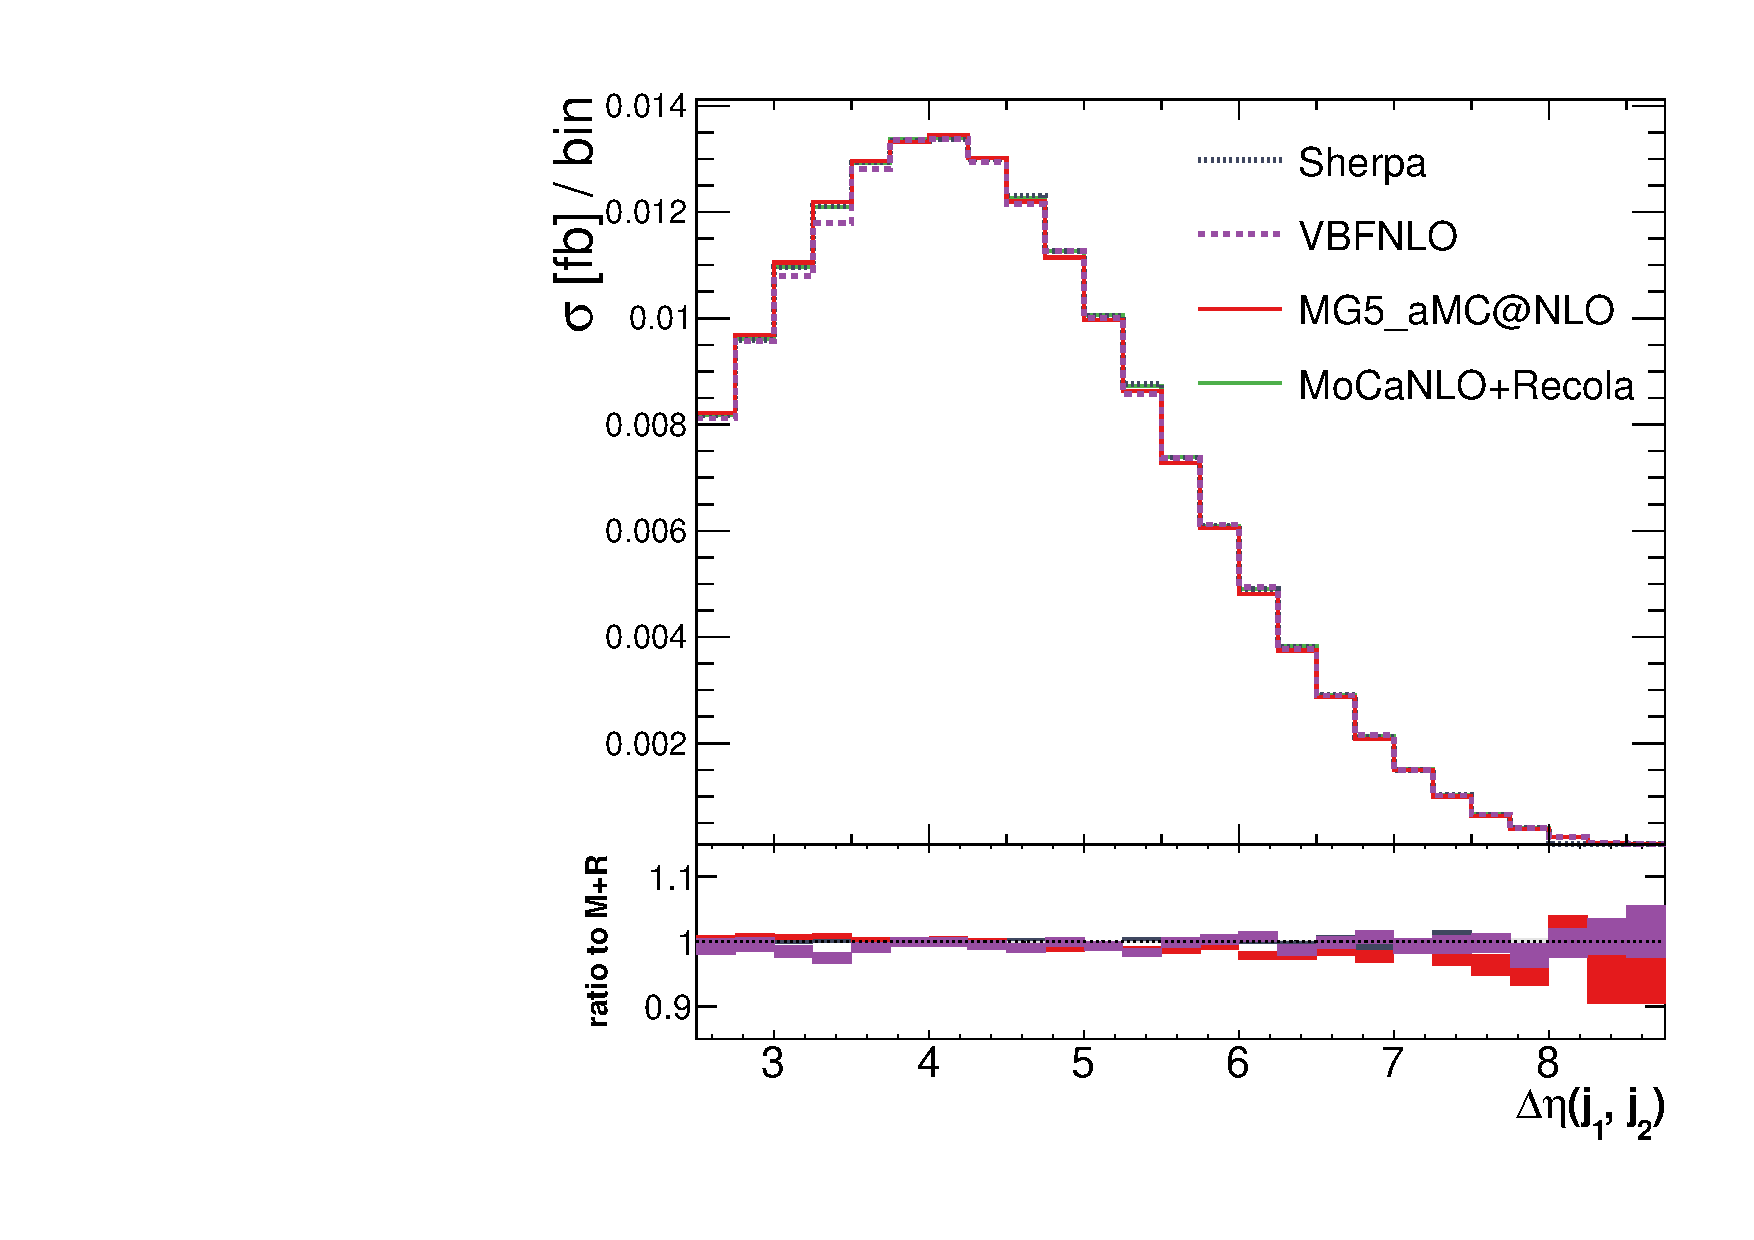
\includegraphics[scale=0.375]{figs/dEtajj_FixedOrder.pdf}
\caption{Differential distributions computed at fixed-order with centre-of-mass energy $\sqrt{s}=13{\rm~TeV}$ at the LHC for ${\rm p} {\rm p}
  \to {\rm e}^-  \nu_{\rm e}  \mu^+ \mu^- {\rm j} {\rm j}$ at LO with fixed scaled $\mu = M_{\rm W}$: 
                invariant mass of the two jets~(left),
                rapidity separation between the two jets~(right).
                The predictions in the lower plot are normalised to the prediction of \MGaMC.
		The shaded bands indicate the relative statistical uncertainty by bin for each sample.
		The statistical uncertainty on the \MGaMC sample is shown in grey, other samples
		are indicated in the ratio with the color indicated in the legend.
                }
\label{vbs_fig_fixed_order}
\end{center}
\end{figure}



Concerning the validation of the VBS approximation ({\sc MoCaNLO}+{\sc Recola} vs. {\sc VBFNLO} for example), both predictions are in good agreement as at the level of the cross section.
This supports the findings of Ref.~\cite{Anders:2018gfr} where preliminary results for similar comparisons for ${\rm W}^\pm{\rm W}^\pm{\rm j}{\rm j}$ have been reported.
This means that the VBS approximation ({\sc VBFNLO}) approximate rather well the full computation ({\sc MoCaNLO}+{\sc Recola}) in the fiducial region chosen.

We stress that such differences of configuration should be considered independently of typical estimates of theoretical uncertainties, especially QCD scale and PDF uncertainties. 
To illustrate this, we compute the PDF uncertainty for the NNPDF3.0 set and the two scale choices considered here. 
The PDF uncertainty is evaluated to be 3--5\% using \MGaMC. 
Scale uncertainties are evaluated using the typical prescription of varying $\mu_{R}$ and $\mu_{F}$ 
subject to the constraint $1/2 \le \mu_{F}/\mu_{R} \le 2$, using \MGaMC and cross-checked with \MoCaNLO+\Recola, 
and are found to be between 7--10\% for the scale choices considered. The full results obtained with \MGaMC are shown in Table~\ref{table:xsecWithUnc}

\begin{table}[htbp]
\begin{center} 
\begin{tabular}{ c | c | c }
 Scale choice & ${\rm p} {\rm p} \to {\rm e}^+  \nu_{\rm e}  \mu^+ \mu^- {\rm j} {\rm j}$  & ${\rm p} {\rm p} \to {\rm e}^-  \bar \nu_{\rm e}  \mu^+ \mu^- {\rm j} {\rm j}$  \\
  \hline\hline
  $\mu_{R} = \mu_{\rm fix} = m_{\mathrm{W}}$                     & $0.286^{+9.2\%}_{-7.8\%} \pm 3.7\%$  & $0.166^{+9.0\%}_{-7.7\%} \pm 4.3\%$ \\
  $\mu = \mu_{\rm dyn} = {\rm Max}\left[p_{\rm T, j}\right]$ & $0.255^{+8.0\%}_{-6.9\%} \pm 3.7\%$  & $0.149^{+9.0\%}_{-7.7\%} \pm 4.3\%$  \\
  \hline
\end{tabular}
\end{center}
\caption{
Fiducial cross sections at LO for the process ${\rm p}{\rm p}\to{\rm e}^+\nu_{\rm e}\mu^+\mu^-{\rm j}{\rm j}$ and ${\rm p}{\rm p}\to{\rm e}^-\bar\nu_{\rm e}\mu^+\mu^-{\rm j}{\rm j}$ at order $\mathcal{O} (\alpha^6)$ 
  via \MGaMC.
The predictions are expressed in fb and are for the LHC running at a centre-of-mass energy of $\sqrt{s}=13 {\rm~TeV}$.
  Uncertainties are expressed as $\sigma^{+\delta_{\mathrm{scale}}}_{-\delta{\mathrm{scale}}} \pm \mathrm \delta_{\mathrm{PDF}}$.
}
\label{table:xsecWithUnc}
\end{table}

We also compare the effect of configurations changes using the general-purpose generators {\sc Sherpa} and \MGaMC. 
These generators are able to compute arbitrary processes in the standard model, 
and therefore have default configurations designed to cover a wide range of processes. It is thus advisable
to explicitly configure settings most appropriate to the process considered. 

Using the same fiducial definition, but with the default parameter settings (defined in param\_card.dat) for 
\MGaMC, we obtain a cross section of 0.1561(5) fb for the ${\rm Max}\left[p_{\rm T, j}\right]$
scale, an increase of 4\% on our nominal value. The primary source of this difference is the 
settings of the boson masses and widths, which are set to their LO values by default in \MGaMC.
Such a setting can be considered appropriate in cases where the partial widths of many decay channels
must be considered together, but for an explicitly leptonic process we argue that the best measured values are
more appropriate.\MP{I don't agree with this. It is just some old default of MG and because they mostly do on-shell computations.}
We do not believe that this $4\%$ difference constitutes an additional uncertainty, but warn that
careful configuration of such parameters should be considered.

We similarly study the default dynamical scale choices in {\sc Sherpa} and \MGaMC. In both cases,
this choice is motivated by a desire for broad application to a variety of processes. Sherpa uses the inverted
parton shower to cluster the matrix element onto a core $2 \to 2$ process. This procedure determines the scales
and is especially suited for truncated shower merging. For \MGaMC,
the default scale depends on the order of the process and shower settings. At LO without
merging of parton multiplicities, the scale is set to the central $m_{T}$ scale after k$_t$-clustering of the event \MP{Should it not be anti-kt?}.
The resulting cross section is $5\%$ greater than the ${\rm Max}\left[p_{\rm T, j}\right]$ result.
Using both the default scale and parameter settings (note however, that we still specify the PDF)
we obtain a value of $\sigma_{\mathrm{default}}) = 0.1638(5)$ fb, $9\%$ greater than our configured
$\mu = {\rm Max}\left[p_{\rm T, j}\right]$ value. We reiterate that this difference, which is
of comparable size to the phenomenological uncertainties, should not necessarily be considered on equal footing.
The fact that the functional form of the dynamical scale choice can have a significant impact compared to the
usual factor of two variation around a nominal value is well established. One should therefore take care
to select an appropriately motivated choice. Additional uncertainties may be appropriate,
but should be considered with care rather than taking a broad envelope of less motivated choices.
This comparison additionally highlights the advantage of the reduced scale dependency at NLO-QCD accuracy.

\subsubsection*{Comparisons after parton shower}

In Figs.~\ref{vbs_fig_shower_1a} and \ref{vbs_fig_shower_1b}, a comparison of results obtained with different
generators for the process ${\rm p} {\rm p} \to {\rm e}^-  \nu_{\rm e}  \mu^+ \mu^- {\rm j} {\rm j}$ at LO supplemented with parton shower with fixed scaled $\mu =M_W$ is shown. 
In particular, in Fig.~\ref{vbs_fig_shower_1a} several differential distributions are shown:
the invariant mass of the two jets, the rapidity separation between
the two jets, the transverse momentum of the anti-muon--muon system,
and the distance between the two jets. The error band in the plots represents the statistical error of the Monte Carlo predictions.  
The overall picture is that the predictions obtained from {\sc Sherpa}, {\sc VBFNLO}+{\sc PYTHIA8}, and \MGaMC+{\sc PYTHIA8} agree rather well over the whole kinematic range.
On the other hand, the predictions obtained from {\sc VBFNLO}+{\sc HERWIG7} seem to be very different for all type of distributions.
These differences can probably be attributed to the configuration of the sample obtained from {\sc VBFNLO}+{\sc HERWIG7} which should be further investigated.

\begin{figure}[htbp]
\begin{center}
   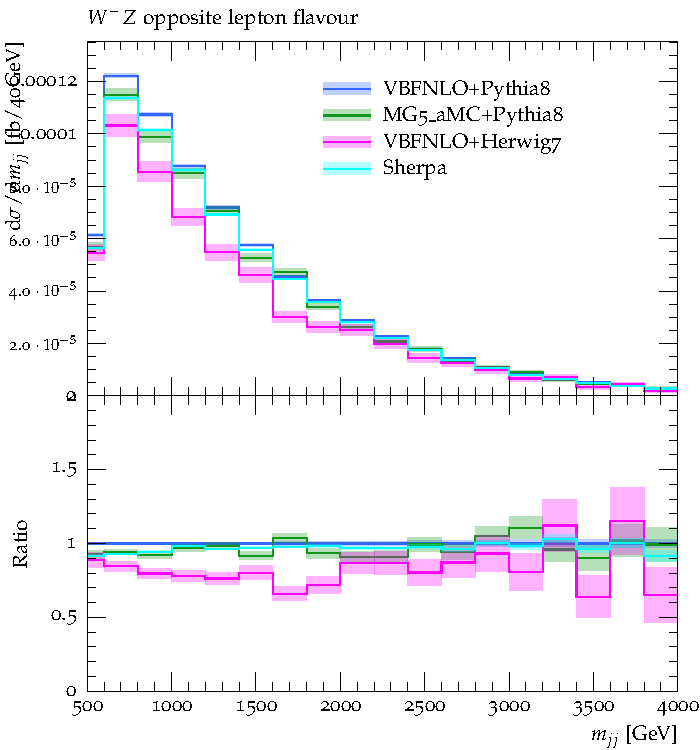
\includegraphics[scale=0.65]{figs/VBFNLO_WmZ_OF_mjj}
   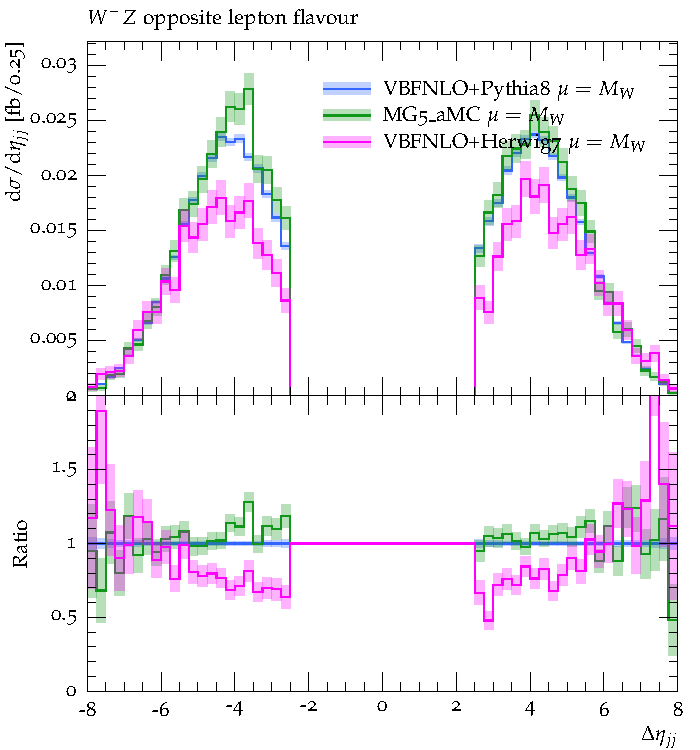
\includegraphics[scale=0.65]{figs/VBFNLO_WmZ_OF_dEtajj}
   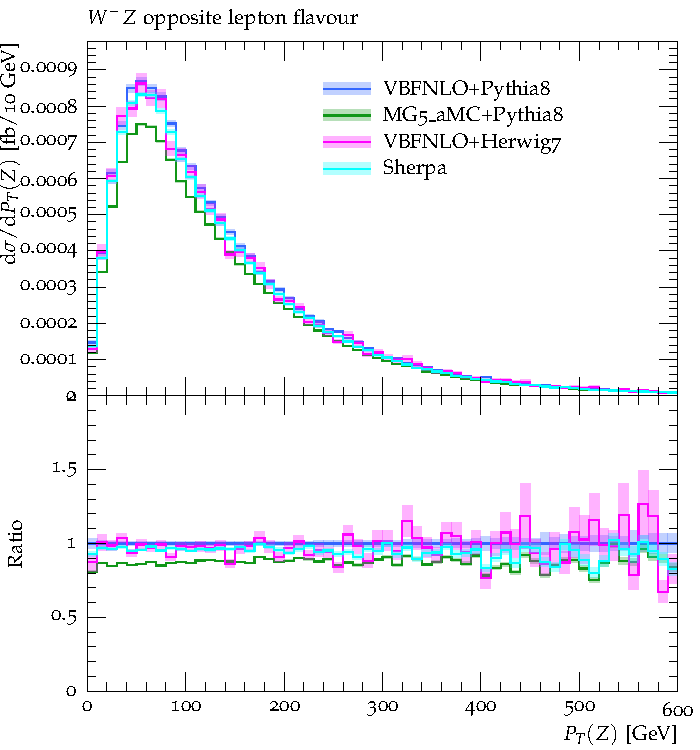
\includegraphics[scale=0.65]{figs/VBFNLO_WmZ_OF_ZPt}
   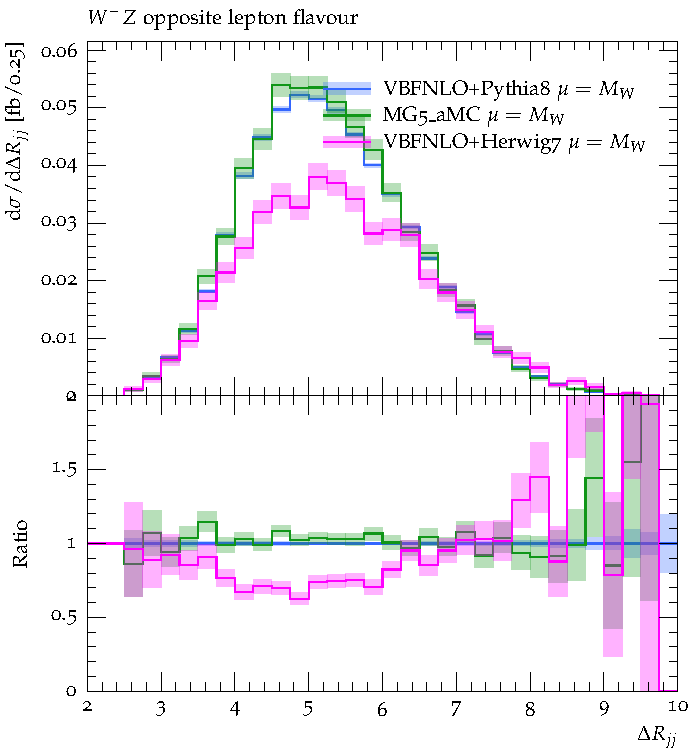
\includegraphics[scale=0.65]{figs/VBFNLO_WmZ_OF_dRjj}
\caption{Differential distributions at a centre-of-mass energy $\sqrt{s}=13{\rm TeV}$ at the LHC for ${\rm p} {\rm p}
  \to {\rm e}^-  \nu_{\rm e}  \mu^+ \mu^- {\rm j} {\rm j}$ at LO with fixed scaled $\mu = M_{\rm W}$: 
                invariant mass of the two jets~(top left),
                rapidity separation between the two jets~(top right)
                transverse momentum of the anti-muon--muon system~(bottom left), and
                distance between the two jets~(bottom right). The error band represents
                the statistical error of the Monte Carlo prediction. }
\label{vbs_fig_shower_1a}
\end{center}
\end{figure}

These differences are more pronounced in Fig.~\ref{vbs_fig_shower_1b} where the Zeppenfeld variable for the three charged leptons and the third jet as well as the number of jets are displayed.
The Zeppenfeld variable for a given particle $X$ is defined as

\begin{equation}
  z_{X} = \frac{y_{X}-\frac{y_{{\rm j}_1}+y_{{\rm j}_2}}2}{|y_{{\rm j}_1}-y_{{\rm j}_2}|} ,
\end{equation}
%
where $y_{{\rm j}_{1/2}}$ are the rapidity of the first and second hardest jet, respectively.
The Zeppenfeld variable of the third jet, as well as the number of jets beyond two, are observables that are not defined at LO,
and are only non-zero thanks to the emissions of the parton shower.
It is thus expected that these feature an even worse agreement than the previously discussed observables, as 
significantly different algorithms are employed by the parton shower generators considered. 
We note that even where there are similarities, we have not taken care to tune the parameters
of the shower but rather consider the spread of predictions as reflective of the uncertainty 
of the parton shower dominated observables. While variables such as the Zeppenfeld of the third jet
have known separation power between the EW and QCD induced production, tuning an experimental selection 
on this observable would introduce large theoretical uncertainties, especially if only LO predictions
are considered. A similar argument holds for a veto on extra jet activity.

\begin{figure}[htbp]
\begin{center}
   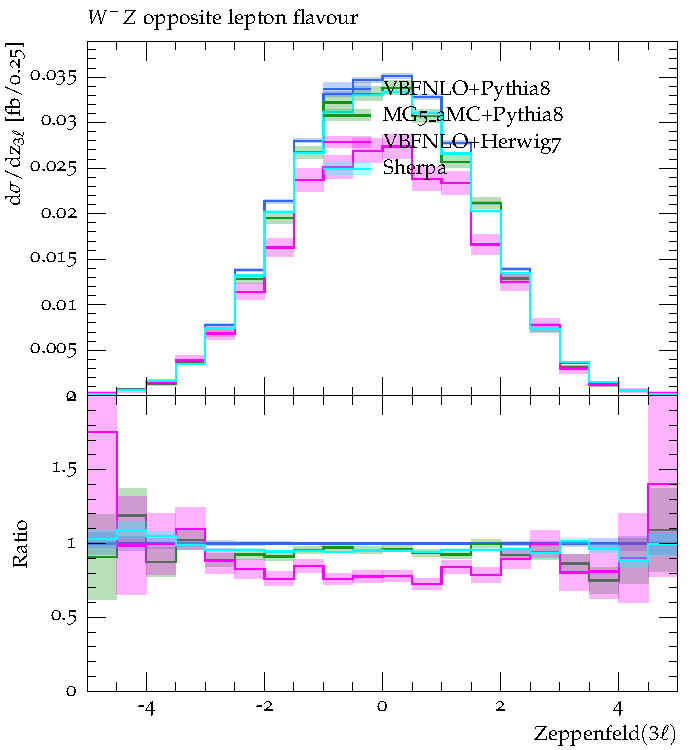
\includegraphics[scale=0.65]{figs/VBFNLO_WmZ_OF_zep3l}
   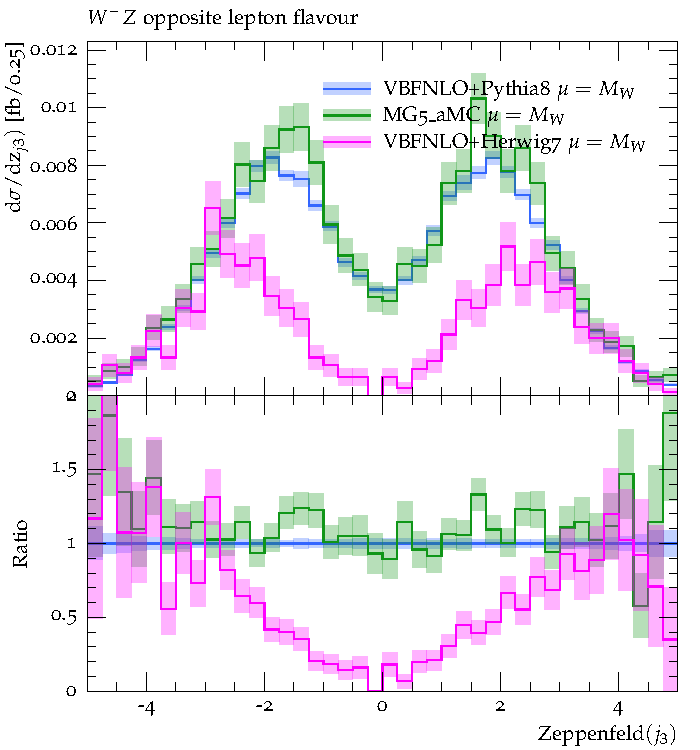
\includegraphics[scale=0.65]{figs/VBFNLO_WmZ_OF_zepj3}
   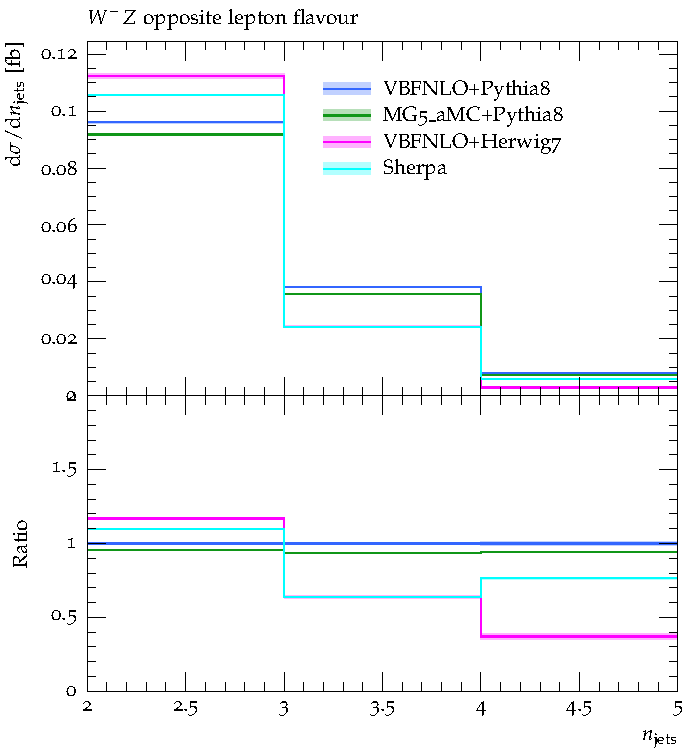
\includegraphics[scale=0.65]{figs/VBFNLO_WmZ_OF_nJets}
\caption{Differential distributions at a centre-of-mass energy $\sqrt{s}=13{\rm TeV}$ at the LHC for ${\rm p} {\rm p}
  \to {\rm e}^-  \nu_{\rm e}  \mu^+ \mu^- {\rm j} {\rm j}$ at LO with fixed scaled $\mu = M_{\rm W}$: 
                Zeppenfeld variable for the three leptons~(top left),
                Zeppenfeld variable for the third jet~(top right)
                number of jets~(bottom). The error band represents
                the statistical error of the Monte Carlo predictions. }
\label{vbs_fig_shower_1b}
\end{center}
\end{figure}

In Figs.~\ref{vbs_fig_shower_2a} and \ref{vbs_fig_shower_2b} results obtained using the fixed scale $\mu = M_{\rm W}$ and dynamic scale $\mu = {\rm Max}\left[p_{\rm T, j}\right]$ are compared.
In particular, predictions for {\sc Sherpa} and \MGaMC for both scales are presented. For
\MGaMC this prediction is obtained by reweighting each event for the difference between the matrix-element calculation
with the fixed scale and the dynamic scale. The statistical uncertainty is therefore largely
correlated between the two predictions for this Monte Carlo.  
The observables displayed are the same as for the previous comparison.
For the invariant mass of the two jets as well as the transverse momentum of the anti-muon--muon system, for both generators, the use of fixed scale enhances the predictions toward high transverse momentum.
For the rapidity separation of the two jets as well as the distance between the two jets, the shape difference between fixed and dynamical scale is not present for \MGaMC.
On the other hand, in {\sc Sherpa}, the use of fixed scale enhances the predictions for small separations.

\begin{figure}[htbp]
\begin{center}
   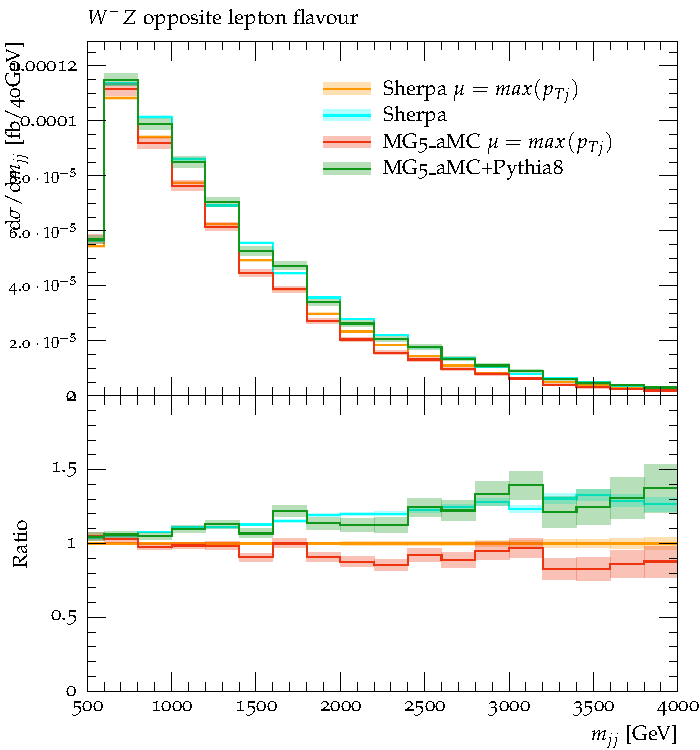
\includegraphics[scale=0.65]{figs/dyn_WmZ_OF_mjj}
   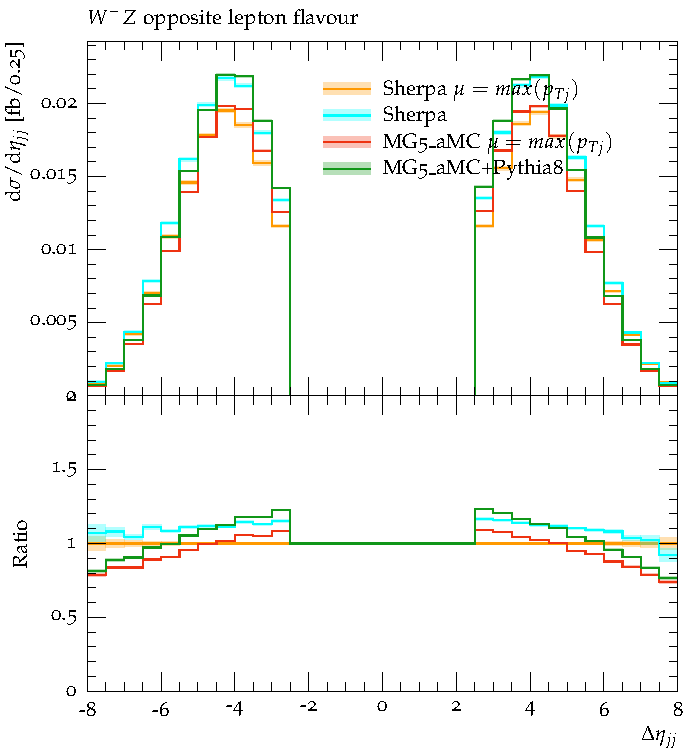
\includegraphics[scale=0.65]{figs/dyn_WmZ_OF_dEtajj}
   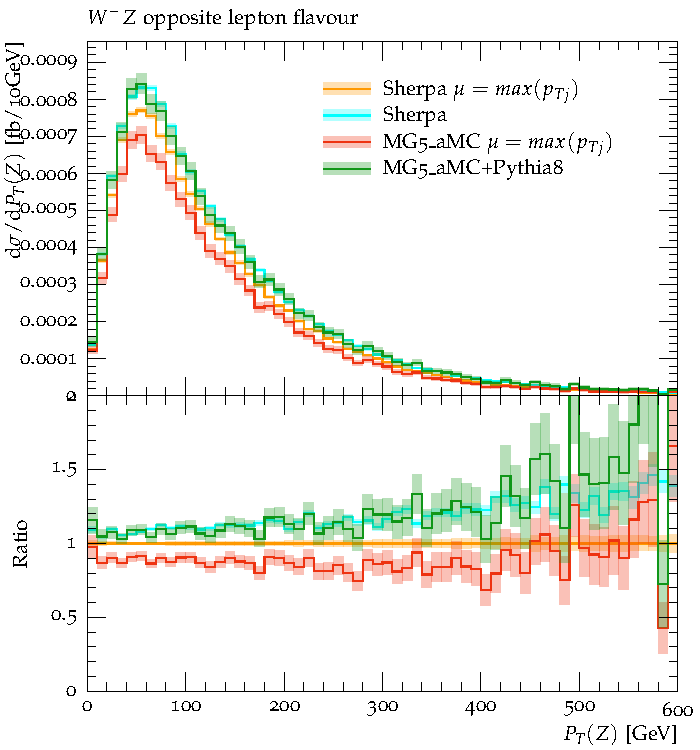
\includegraphics[scale=0.65]{figs/dyn_WmZ_OF_ZPt}
   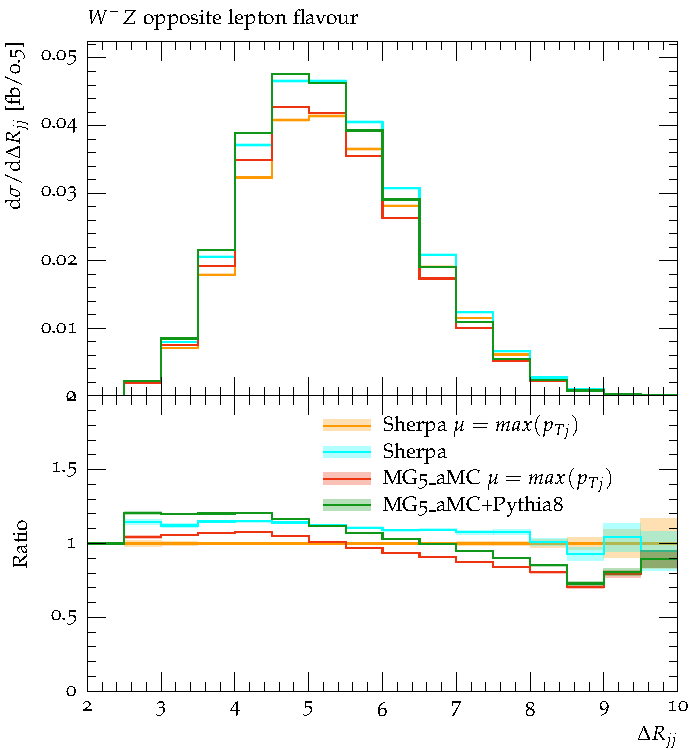
\includegraphics[scale=0.65]{figs/dyn_WmZ_OF_dRjj}
\caption{Differential distributions at a centre-of-mass energy $\sqrt{s}=13{\rm TeV}$ at the LHC for ${\rm p} {\rm p}
  \to {\rm e}^-  \nu_{\rm e}  \mu^+ \mu^- {\rm j} {\rm j}$ at LO with fixed and dynamic scale values:  
                invariant mass of the two jets~(top left),
                rapidity separation between the two jets~(top right)
                transverse momentum of the anti-muon--muon system~(bottom left), and
                distance between the two jets~(bottom right).
                In the lower plots, the predictions are normalised to the prediction of {\sc Sherpa} with
                dynamical scale. The error band represents
                the statistical error of the Monte Carlo predictions. For the two \MGaMC
                calculations this statistical error is largely correlated, as explained in the text.}
\label{vbs_fig_shower_2a}
\end{center}
\end{figure}

Concerning the last set of observables (Zeppenfeld variable of the three leptons and third jet as well as the number of jets) in Fig.~\ref{vbs_fig_shower_2b}, the use of fixed or dynamical scale does not have a large impact.
The only clearly visible difference between fixed and dynamical scale is the normalisation.
This effect is already observed at the level of the fiducial cross section in Tables~\ref{table:xsectLOfix} and \ref{table:xsectLOdyn}.
The effect of the different scale amounts to a change in normalisation of about $12\%$ for both ${\rm p}{\rm p}\to{\rm e}^+\nu_{\rm e}\mu^+\mu^-{\rm j}{\rm j}$ and ${\rm p}{\rm p}\to{\rm e}^-\bar\nu_{\rm e}\mu^+\mu^-{\rm j}{\rm j}$ processes.

\begin{figure}[htbp]
\begin{center}
   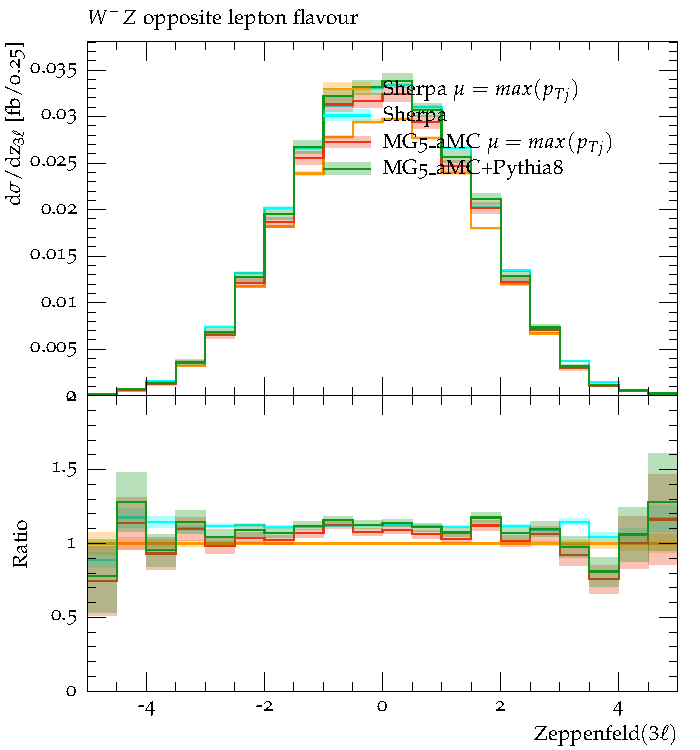
\includegraphics[scale=0.65]{figs/dyn_WmZ_OF_zep3l}
   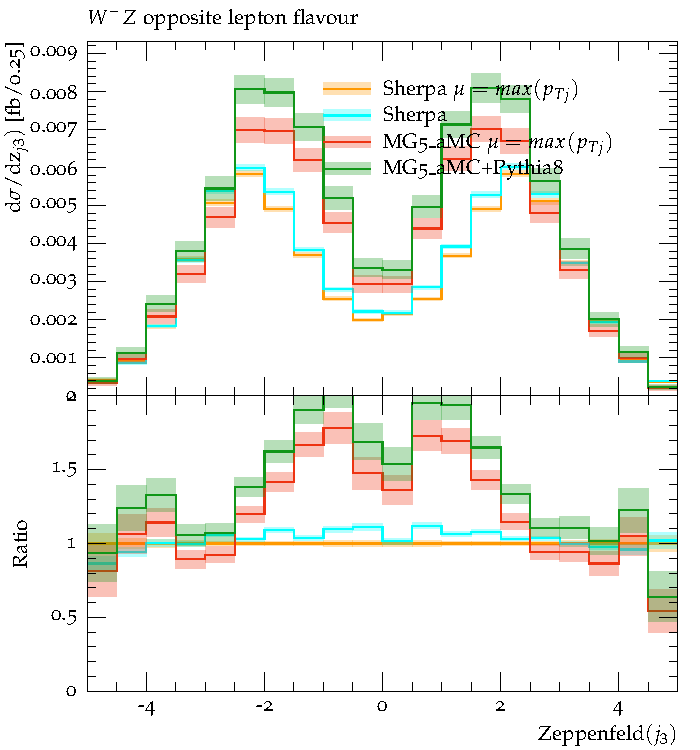
\includegraphics[scale=0.65]{figs/dyn_WmZ_OF_zepj3}
   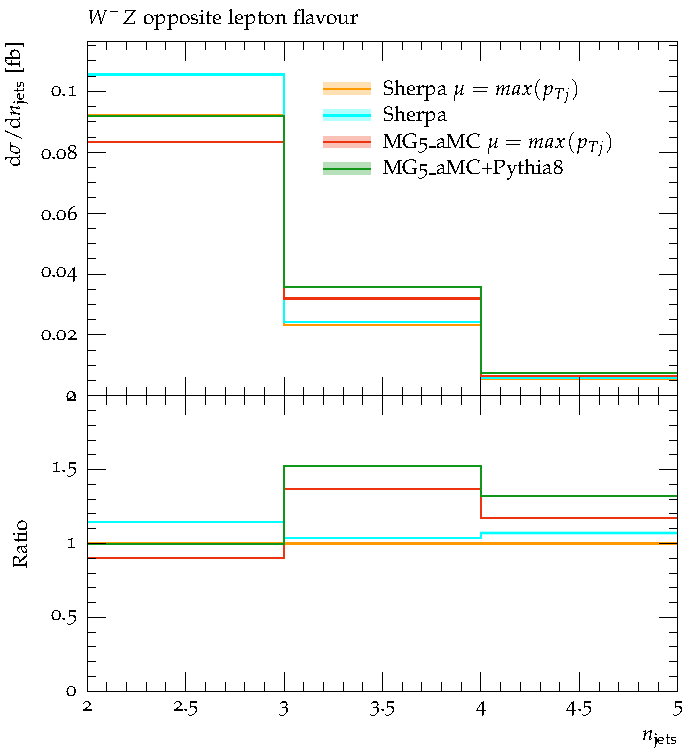
\includegraphics[scale=0.65]{figs/dyn_WmZ_OF_nJets}
\caption{Differential distributions at a centre-of-mass energy $\sqrt{s}=13{\rm TeV}$ at the LHC for ${\rm p} {\rm p} \to {\rm e}^-  \nu_{\rm e}  \mu^+ \mu^- {\rm j} {\rm j}$ at LO with fixed and dynamic scale values: 
                Zeppenfeld variable for the three leptons~(top left),
                Zeppenfeld variable for the third jet~(top right)
                number of jets~(bottom).
                In the lower plots, the predictions are normalised to the predictions of {\sc Sherpa} with dynamical scale. The error band represents
                the statistical error of the Monte Carlo predictions. For the two \MGaMC
                calculations this statistical error is largely correlated, as explained in the text.}
\label{vbs_fig_shower_2b}
\end{center}
\end{figure}

\subsection{Conclusions \label{vbs_concl}}

The measurement of the EW component of the ${\rm p}{\rm p} \to {\rm W}^{\pm}{\rm Z}{\rm j}{\rm j}$ process constitutes a real challenge for experimental collaborations.
Such a measurement is complicated for several reasons including the low cross section and the overwhelming irreducible background.
Therefore, these measurements have to rely on theoretical predictions in order to extract a signal.
This makes theoretical predictions implemented in various Monte Carlo programs very important.
It is thus key to have a good control over these predictions.
To that end we have performed LO comparisons of different theoretical predictions possibly supplemented by parton shower.
The comparisons have all been performed with pre-defined input values and a generic fiducial region for VBS measurements.

The first finding of the present study is that the EW component is overwhelmingly dominated by its irreducible QCD background.
In the fiducial region that we have chosen, $80\%$ of the fiducial cross section in accounted by the QCD background.
This indicates the need for observables that enhance the EW contribution.
Beyond the di-jet invariant mass and the rapidity separation between the two jets, we found that the distance between the two jets could have a good discriminating power.
We also found that interferences between the QCD and EW amplitudes are also negligible in the fiducial region.

In the present proceedings, we have also performed a LO comparison.
At parton level, the agreement between the various theoretical predictions is reasonably good.
This statement holds both for the inclusive cross section and differential distributions.
Nonetheless differences appear.
These can probably be attributed to the misconfiguration of the runs presented here.
On the other hand, the differences between a full computation and a VBS-approximated one are relatively small.
This implies that, as for the ${\rm W}^\pm{\rm W}^\pm{\rm j}{\rm j}$ signature \cite{Anders:2018gfr}, the VBS approximation seems to be good in the typical fiducial regions used by experimental collaborations for their measurements.

The predictions at LO supplemented with parton shower have relied on the fixed-order configuration.
No tuning of the parton shower parameters have been performed and the default values have been taken.
For {\sc PYTHIA8}, the {\sc CUETP8M1} tune \cite{Khachatryan:2015pea} which is based on the Monash tune \cite{Skands:2014pea} has been used. 
The agreement is in general worse, in particular for observables that are defined only beyond LO, the theoretical predictions diverge significantly.
Concerning the role of the fixed and dynamical scales, we have found that they can have a rather large influence on the predictions for the inclusive cross section and differential distributions.
This indicates that the inclusion of higher order predictions may cure this behaviour.

Finally, we would like to stress that these results constitute only a preliminary study of theoretical predictions for the process ${\rm p}{\rm p} \to {\rm W}^{\pm}{\rm Z}{\rm j}{\rm j}$.
In particular, strictly fixed-order computation are expected to give a much better agreement.
At the level of parton shower, several differences appear and these are not yet fully investigated.
This demonstrates the difficulty to obtain consistent Monte Carlo predictions.
In particular, the choice of inputs and configuration can have a large impact on physics results.
NLO QCD and EW effects have not been studied in this work.
They should play a significant role in theoretical predictions for VBS and should be taken into account as much as possible in future studies.
This study thus warrants further efforts in all the above mentioned directions that could not be covered here.

%\clearpage
\bibliography{vbs_bib}

\end{document}
